\documentclass{standalone}
\usepackage{tikz}

% Making a DAG
\usepackage{tkz-graph}  
\usetikzlibrary{shapes.geometric}
\tikzstyle{VertexStyle} = [shape            = ellipse,
                               minimum width    = 6ex,%
                               draw]
 \tikzstyle{EdgeStyle}   = [->,>=stealth']      

\begin{document}

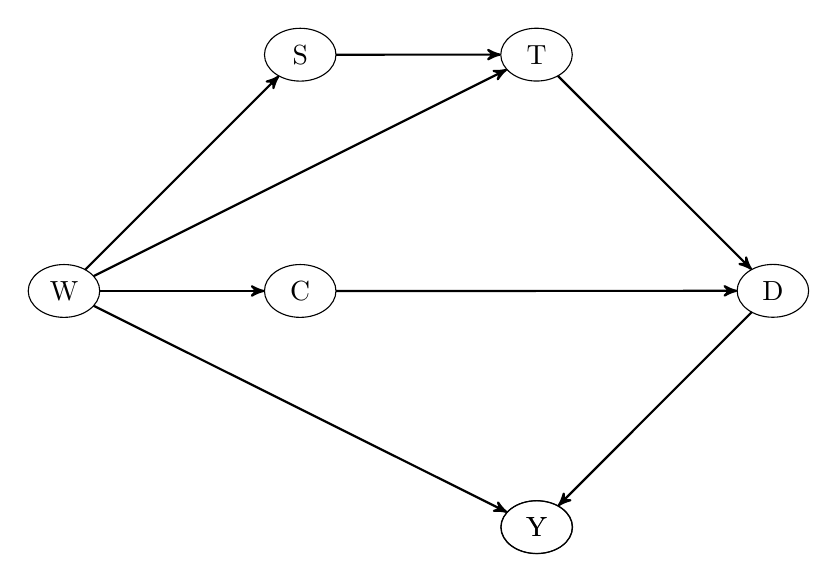
\begin{tikzpicture}[scale=1.5] 
\SetGraphUnit{2} 
\Vertex{W}  \NOEA(W){S} \EA(S){T}  \EA(W){C} \SOEA(T){D} \SOEA(C){Y} \SOWE(D){Y}
\Edges(W, S, T) \Edges(W,T) \Edges(W, C) \Edges(T, D) \Edges(C, D) \Edges(W, Y) \Edges(D, Y)
\end{tikzpicture}

\end{document}